\subsection{Dolní a pásmová propust 2. řádu, 4. řádu}\label{s:DP2}
Dolní propust druhého řádu má přenos v nekonečnu nulový $H_{\infty} = 0$. Přenosová funkce je
\begin{equation}
H(j\omega) = \frac{H_0 \omega_c ^2}{(j\omega)^2 + \frac{\omega _c}{Q}(j\omega) + \omega _c ^2}.
\end{equation}
\noindent Obvodová simulace byla realizována v programu Multisim. Bylo zvoleno symetrické napájení OZ $V_{DD},V_{SS} = \pm 15$ V. Regulací vstupního proudu je ovlivňován pracovní bod obvodu (mezní kmitočet). Vstupní externí proud $I_{ABC} = 0.5$ $\mu$A byl zvolen tak, aby byl obdržen mezní kmitočet cca 100 kHz. Externím proudem $I_{ABC} \in$ $[5$ $\mu$A ; 500 $\mu$A] je garantováno minimální výstupní napětí $U_{OUT} = \pm 12$ V, standardně $V_{peak 1} = 14.2$ V a $V_{peak 2} = -14.4$ V. Při výstupním napětí v tomto intervalu je šum vzhledem k signálu zanedbatelný a nezkreslí výsledky simulace.\\
\noindent Bylo použito zapojení s paralelně řazeným uzemněným kapacitorem, odporem a indukčností (RLC rezonanční obvod), kde $R = 1/g_m$ a $L = C/(g_{m1}g_{m2})$ a vstupní proud $I = g_mV$. Podobně jako v sekci \ref{s:ODV} bylo obrženo analogií k pasivnímu obvodu
\begin{align}
\frac{V_{BP}}{g_{m3}V_i} &= \frac{1}{pC + g_m^2/(pC) + g_{m3}}\\
\frac{V_{BP}}{V_i} &= \frac{pg_{m3}C}{p^2C^2 + pg_{m3}C + g_m^2}.
\end{align}
\begin{figure}[h]
\centering
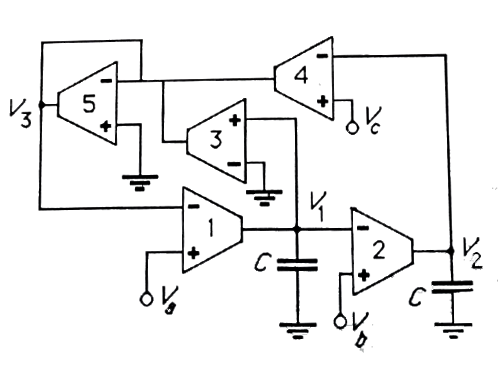
\includegraphics[scale=0.55]{biquad.png}
\caption[Obecná OTA struktura pro bikvad]{Obecná OTA struktura pro bikvad \cite{12} \label{s:BIK}}
\end{figure}
\noindent Zapojení je popsáno na obrázku \ref{s:BIK}. Zesilovače 1 a 2 pracují jako invertující integrátory, zbývající zesilovače vytvářejí kladnou a zápornou zpětnou vazbu z výstupu integrátorů vedoucí na sčítací vstup. Znaménko vazby je určeno volbou vstupní svorky zesilovačů 3 a 4. Výstupy obvodu jsou napěťové (na výstupu sumačního zesilovače 5, resp. integrátoru 1 a 2). Buzení může být proudové (v obrázku \ref{s:BIK} na místě $V_1$ a $V_2$) nebo napěťové s využitím vstupních svorek transkonduktančních zesilovačů. Uvažováním napětí $V_a, V_b, V_c$ na obrázku \ref{s:BIK} jako vstupy byly obdrženy výstupní napětí
\begin{align}
V_1 &= \frac{pC_2g_{m1}(g_{m5}V_a - g_{m4}V_c) + g_{m1}g_{m2}g_{m4}V_b}{D(s)}\\
V_2 &= \frac{(pC_1g_{m2}g_{m5} + g_{m1}g_{m2}g_{m3})V_b + g_{m1}g_{m2}(g_{m4}V_c - g_{m5}V_a)}{D(s)}\\
V_3 &= \frac{p^2C_1C_2g_{m4}V_c + p(C_2g_{m1}g_{m3}V_a - C_1g_{m2}g_{m4}V_b) + g_{m1}g_{m2}g_{m4}V_a}{D(s)},
\end{align}\label{s:V3}
kde
\begin{equation}
D(p) = C_1C_2g_{m5}(p^2 + p\frac{1}{C_1}\frac{g_{m1}g_{m3}}{g_{m5}} + \frac{g_{m1}g_{m2}g_{m4}}{C_1C_2g_{m5}}).
\end{equation}\label{s:DS}
\noindent Zvolením $V_a = V_b = 0$ a $V_c = V_i$ byly obdrženy následující přenosové funkce
\begin{align}
H_{BP}(p) &= \frac{V_1}{V_i} = - \frac{sC_2g_{m1}g_{m4}}{D(s)}\\
H_{LP}(p) &= \frac{V_2}{V_i} = \frac{g_{m1}g_{m2}g_{m4}}{D(s)}\\
H_{HP}(p) &= \frac{V_3}{V_i} = \frac{s^2C_1C_2g_{m4}}{D(s)},
\end{align}
kde $D_s$ odpovídá rovnici \ref{s:DS}.\\
Obecná přenosová funkce bikvadu může být obdržena položením $V_a = V_b = V_c = V_i$ a úpravami vztahu \ref{s:V3} bylo obdrženo
\begin{equation}
\frac{V_3}{V_i} = \frac{p^2C_1C_2g_{m4} + p(C_2g_{m1}g_{m3} - C_1g_{m2}g_{m4}) + g_{m1}g_{m2}g_{m4}}{D(s)}.
\end{equation}
\noindent 
V simulaci byl dle výše popsaných poznatků na výstupu 2. OTA (V1) obdržen filtr typu PP 1. řádu s poklesem 20 dB/dek a na výstupu 3. OTA (V2) DP 2. řádu s poklesem 40 dB/dek.
\begin{figure}[h]
\centering
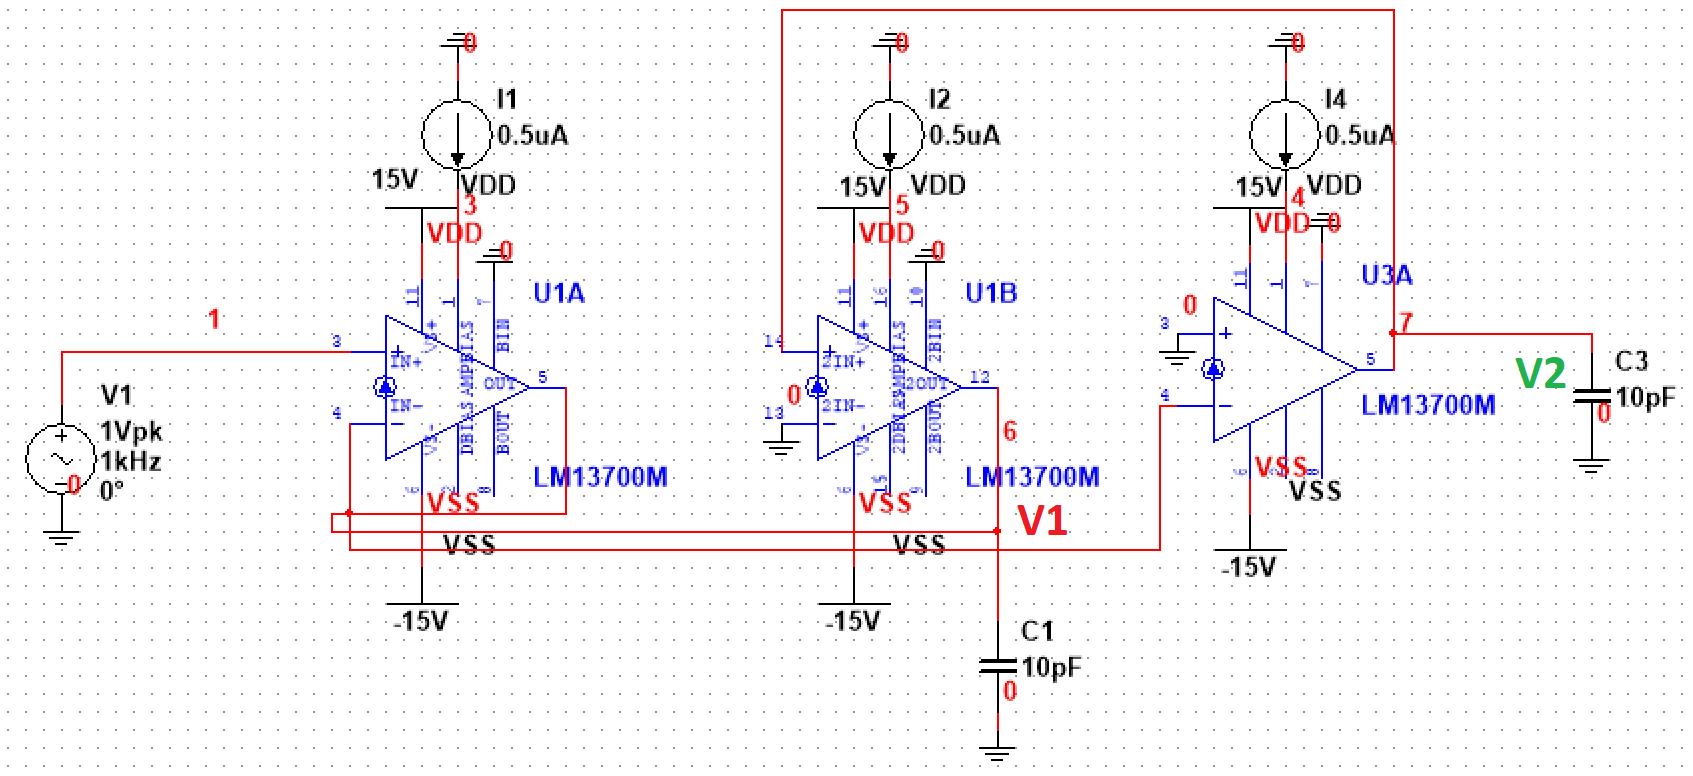
\includegraphics[scale=0.3]{bplp.png}
\caption{Schéma zapojení DP 2. řádu}
\end{figure}
\begin{figure}[h]
\centering
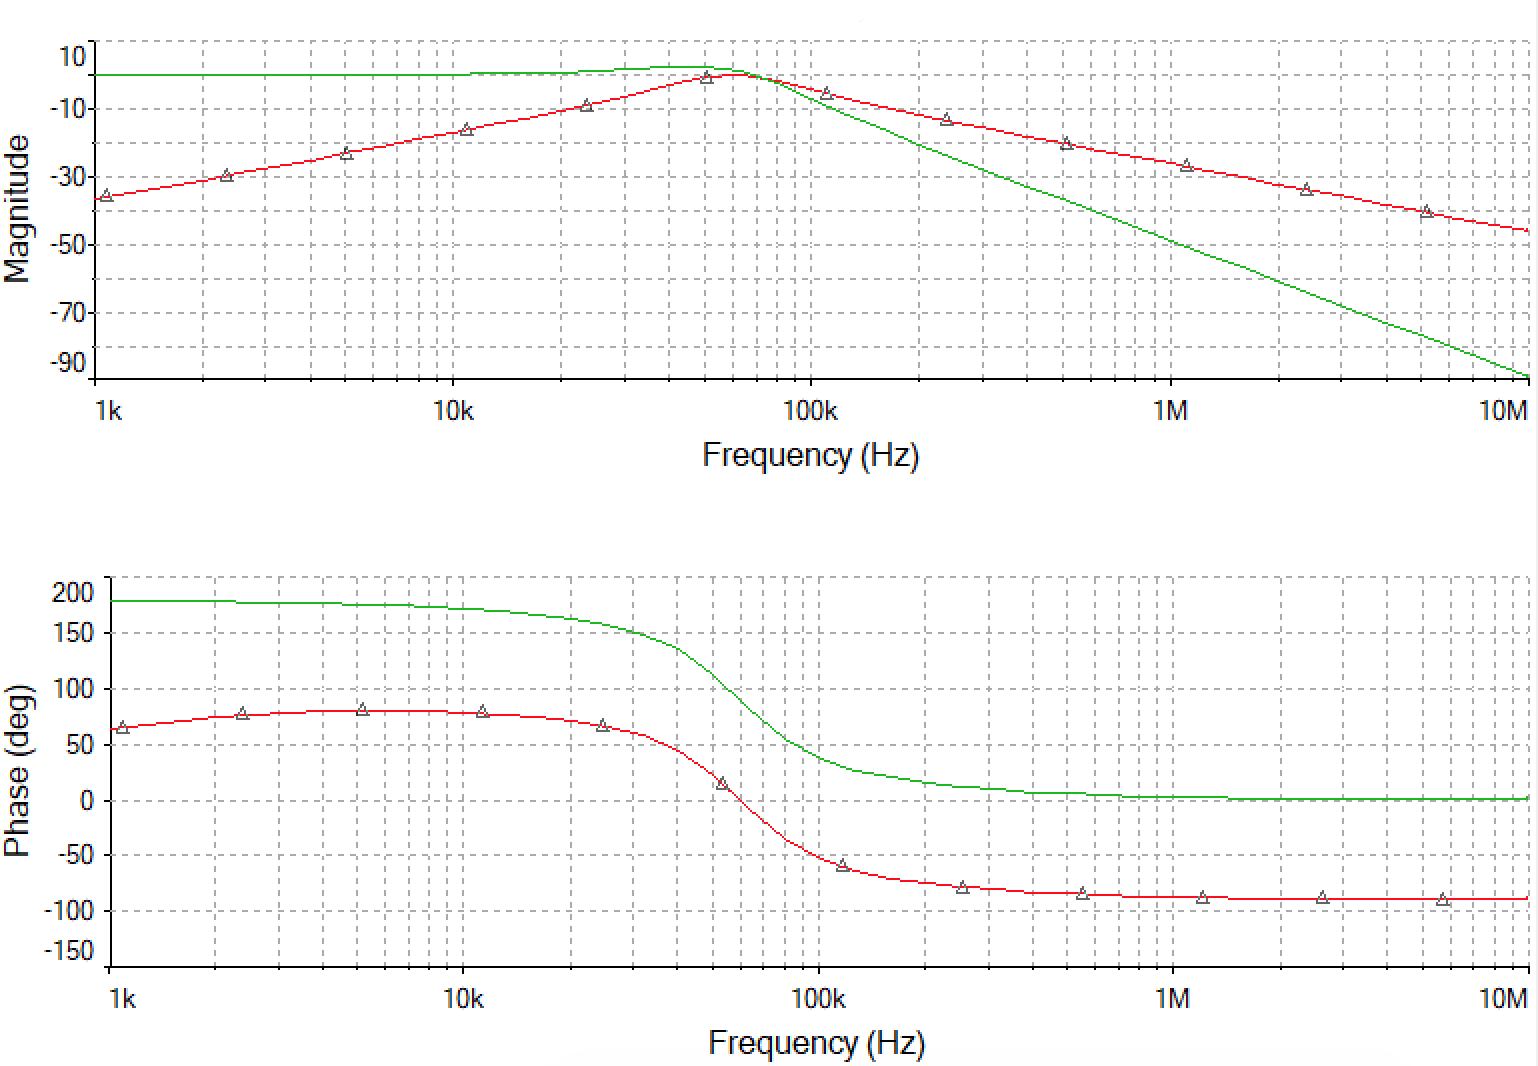
\includegraphics[scale=0.5]{bplp2.png}
\caption{Amplitudová a fázová charakteristika DP 2. řádu, PP 1. řádu}
\end{figure}
\noindent V případě realizace těchto základních přenosů (PP, DP) lze zapojení dále zjednodušit až na obvod obsahující pouze 3 zesilovače, viz obrázek \ref{s:BIK2}. Přenos tohoto obvodu s výstupem pořadě v bodu D a P je dán rovnicemi
\begin{align}
U_D(p) &= \frac{p\frac{g_{m3}U_3-g_{m2}U_2}{C_2}+\frac{g_{m1}g_{m2}}{C_1C_2}U_1}{p^2 + p\frac{g_{m3}}{C_2} + \frac{g_{m1}g_{m2}}{C_1C_2}}\\
U_P(p) &= \frac{p\frac{g_{m1}}{C_1}U_1 + \frac{g_{m1}}{C_1C_2}(g_{m3}U_1+g_{m2}-g_{m3}U_3)}{p^2 + p\frac{g_{m3}}{C_2} + \frac{g_{m1}g_{m2}}{C_1C_2}}.
\end{align}
\noindent Elementárními úpravami lze tyto rovnice zjednodušit na
\begin{align}
U_D(p) &= \frac{pC_1(g_{m3}U_3 - g_{m2}U_2) + g_{m1}g_{m2}U_1}{p^2C_1C_2 + pC_1g_{m3} + g_{m1}g_{m2}}\\
U_P(p) &= \frac{pC_2g_{m1}U_1 + g_{m1}(g_{m3}U_1 + g_{m2} - g_{m3}U_3)}{p^2C_1C_2 + pC_1g_{m3} + g_{m1}g_{m2}}.
\end{align}
\noindent
\begin{figure}[h]
\centering
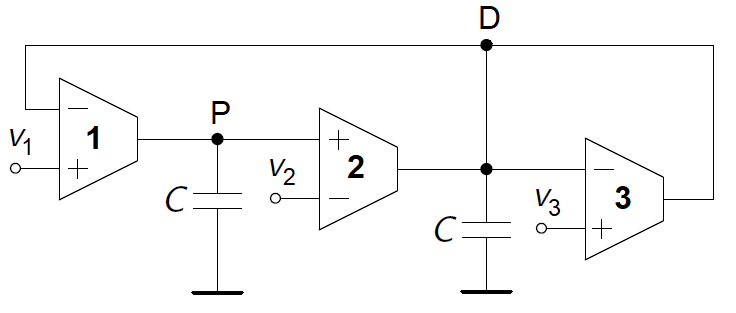
\includegraphics[scale=0.075]{biquad1.png}
\caption[Zjednodušená verze bikvadu OTA-C]{Zjednodušená verze bikvadu OTA-C \cite{3} \label{s:BIK2}}
\end{figure}
\noindent K sestavení dolní propusti 4. řádu bylo použito kaskádní zapojení sestávající ze sériově zapojených bloků. Přenosové funkce jednotlivých bloků se násobí
\begin{equation}
H_k(j\omega) = \frac{U_k (j\omega)}{U_{k-1}(j\omega)}.
\end{equation}
Přenos posledního bloku je dán vztahem
\begin{equation}
H_{1 \rightarrow k}(j\omega) = \frac{U_k (j\omega)}{U_{in}(j\omega)} = \prod _{n=1}^{k} H_n(j\omega).
\end{equation}
\begin{figure}[h]
\centering
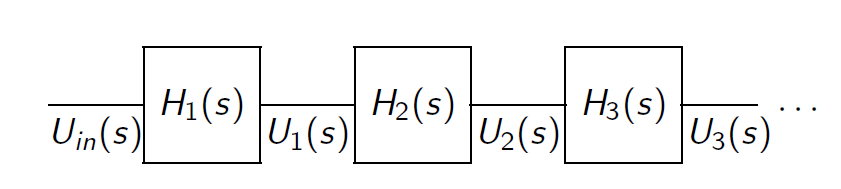
\includegraphics[scale=0.4]{schemata.png}
\caption[Kaskádní zapojení]{Kaskádní zapojení \cite{5}}
\end{figure}
Kaskádním zapojením dvou dolních propusti ze sekce \ref{s:DP2} byl obdržen filtr 4. řádu s poklesem 80 dB/dek.
\begin{figure}[h]
\centering
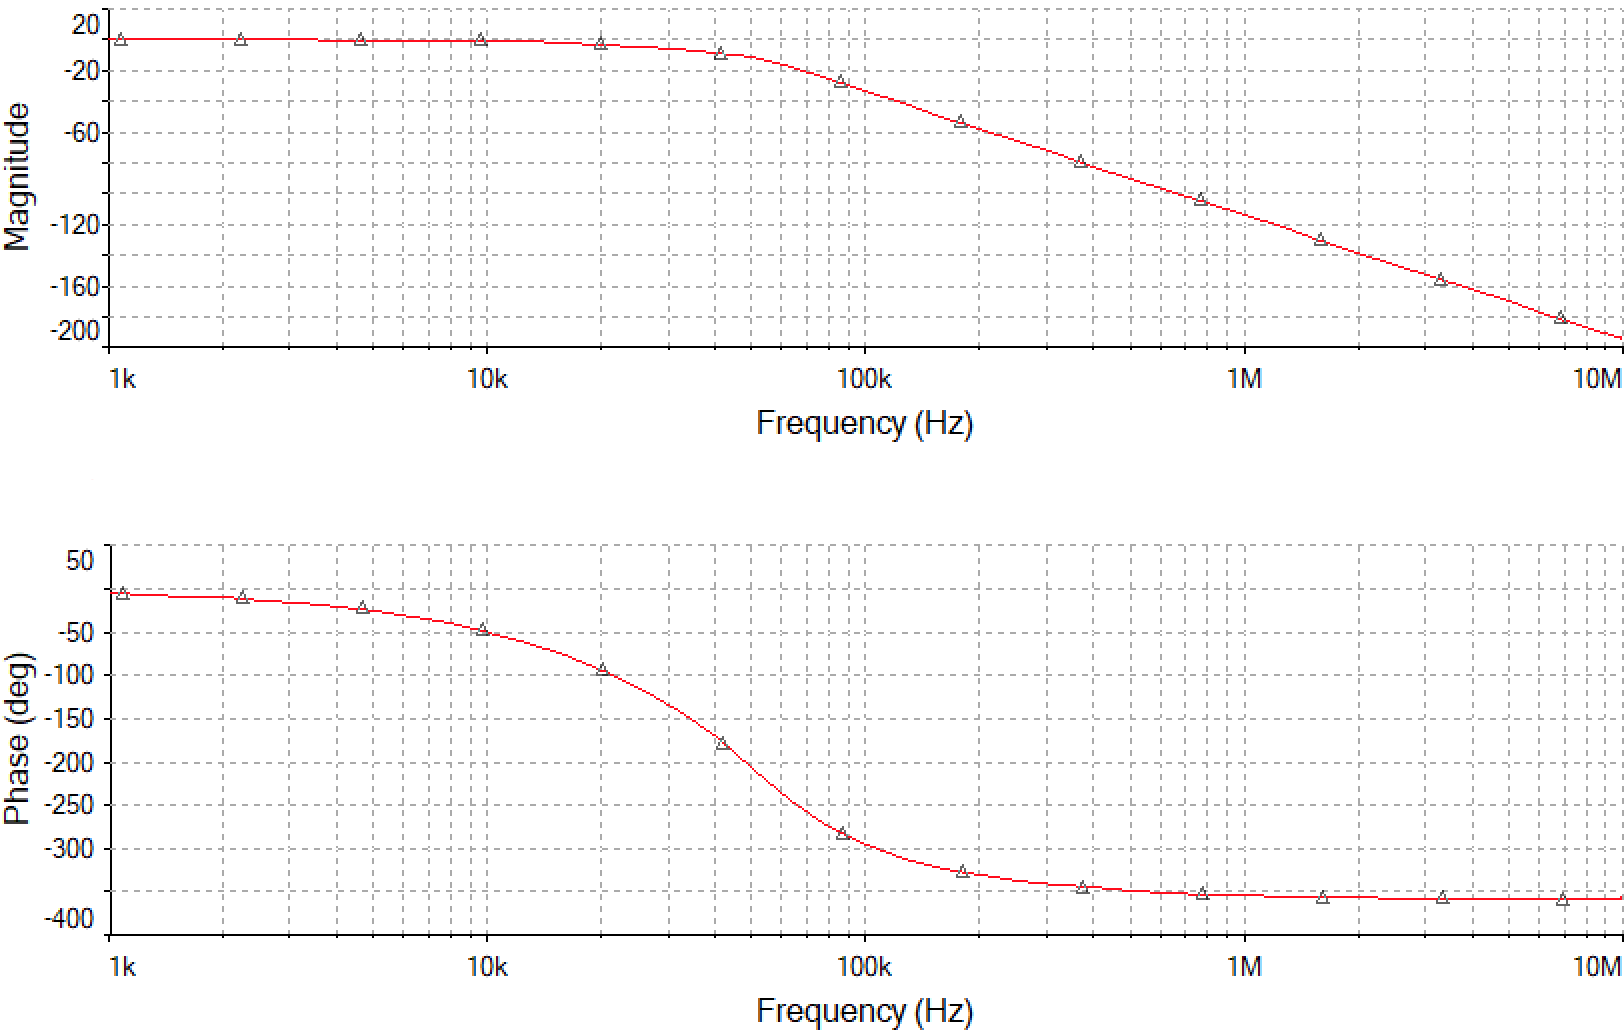
\includegraphics[scale=0.45]{bplp3.png}
\caption{Amplitudová a fázová charakteristika DP 4. řádu}
\end{figure}
\noindent Pásmovou propust lze získat zapojením dolní a horní propusti.\\
Horní propust druhého řádu má přenos v nule nulový $H_{0} = 0$. Přenosová funkce je
\begin{equation}
H(j\omega) = \frac{H_{\infty} (j\omega) ^2}{(j\omega)^2 + \frac{\omega _c}{Q}(j\omega) + \omega _c ^2}.
\end{equation}
\begin{figure}[h]
\centering
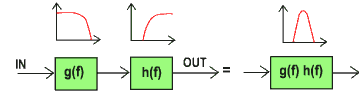
\includegraphics[scale=0.9]{fig9.png}
\caption[Násobení přenosů]{Násobení přenosů \cite{13}}
\end{figure}
\noindent Pásmová propust má přenos v nule i nekonečnu nulový $H_{0} = H_{\infty} = 0$. Přenosová funkce je
\begin{equation}
H(j\omega) = \frac{H_{B} \frac{\omega _c}{Q} (j\omega) }{(j\omega)^2 + \frac{\omega _c}{Q}(j\omega) + \omega _c ^2}.
\end{equation}
\begin{figure}[h]
\centering
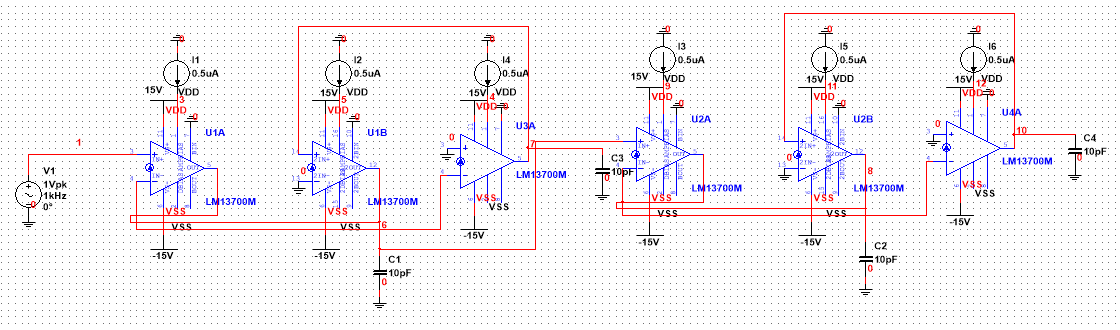
\includegraphics[scale=0.6]{PP2O.png}
\caption{Schéma zapojení DP 4. řádu, PP 2. řádu}
\end{figure}
\begin{figure}[h]
\centering
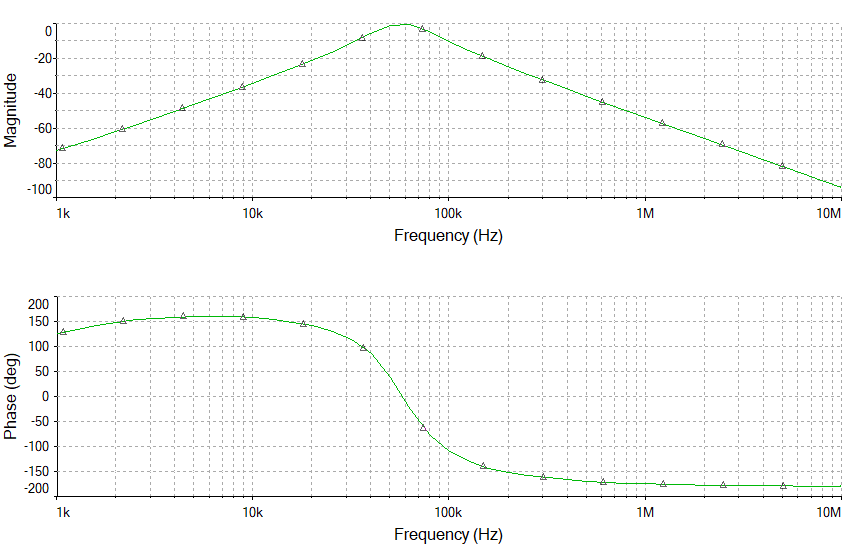
\includegraphics[scale=0.6]{PP2O2.png}
\caption{Amplitudová a fázová charakteristika PP 2. řádu}
\end{figure}
\noindent Kaskádním zapojením dvou PP 2. řádu byla obdržena PP 4. řádu s poklesem 80 dB/dek. Zapojení spočívá ve spojení dvou integrátorů, přičemž jeden z nich je neinvertující ztrátový a druhý invertující bezeztrátový.
\begin{figure}[h]
\centering
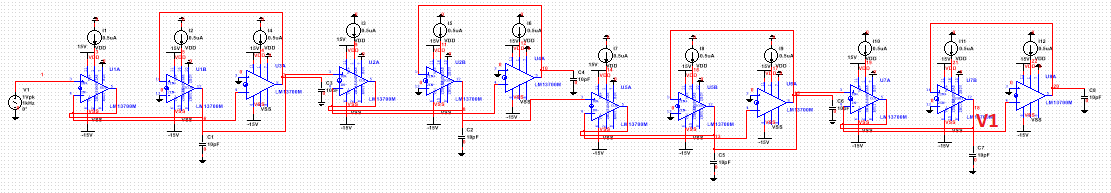
\includegraphics[scale=0.5]{PP4O.png}
\caption{Schéma zapojení PP 4. řádu}
\end{figure}
\begin{figure}[h]
\centering
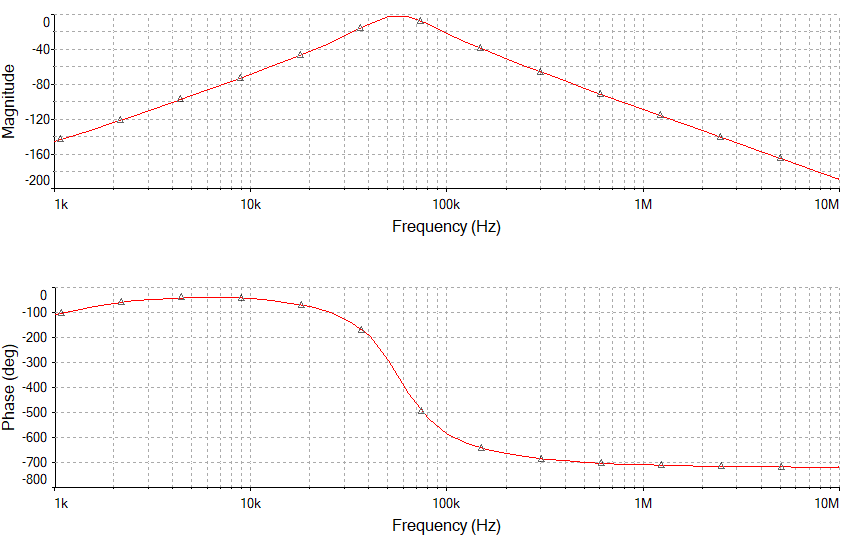
\includegraphics[scale=0.6]{PP4O2.png}
\caption{Amplitudová a fázová charakteristika PP 4. řádu}
\end{figure}